% =====================================================================
%  Основное содержимое отчёта.
% =====================================================================

\labpart{Структура разработанной системы}

Машинный перевод реализован как новый сценарий использования поверх
архитектуры ЛР1--ЛР3 (см. \texttt{docs/ARCHITECTURE.md}): границы
сервисов по-прежнему проведены по зоне ответственности, а не по
лабораторной работе. В отличие от ЛР2 (\texttt{lang-id-service}) и ЛР3
(\texttt{summarization-service}), для ЛР4 не понадобился отдельный
микросервис -- перевод по словарю и синтаксический разбор предложения
являются такими же операциями «текст на входе -- разбор spaCy -- чистый
результат на выходе», как токенизация и лемматизация, поэтому они
естественно легли в уже существующий \texttt{nlp-service}, а хранение
словаря и истории переводов -- в уже существующий \texttt{api}.
Структура системы на уровне контейнеров (C4, уровень 2) показана на
рисунке~\ref{fig:architecture-c4}; связи, добавленные именно в этой
лабораторной работе, выделены зелёным цветом.

\pumldiagram{architecture-c4}{Диаграмма контейнеров разработанной системы (нотация C4); зелёным -- новое в ЛР4}{architecture-c4}{0.95}

\texttt{nlp-service} получил два новых эндпоинта: \texttt{POST
/translate} (пословный перевод текста по переданному словарю плюс
частотный список слов для вкладки~1) и \texttt{POST /syntax/parse}
(дерево синтаксического разбора одного предложения для вкладки~2).
Оба эндпоинта, как и остальные операции \texttt{nlp-service}, не
хранят состояние и не обращаются к БД -- словарь передаётся в запросе,
а результат возвращается как чистая функция входа. Оркестрацией (кто
и когда обращается к словарю, что сохранить в БД) занимается
\texttt{api}, как и для остальных сценариев системы: новый модуль
\texttt{application/translation} загружает актуальный словарь из
БД, вызывает \texttt{nlp-service} и сохраняет результат.

Помимо этого, ЛР4 расширила ответственность \texttt{frontend}:
\begin{itemize}
  \item новая страница «Перевод» с четырьмя вкладками -- собственно
  перевод, частотный словарь (вкладка~1 методички), синтаксический
  разбор предложения (вкладка~2) и утилита пополнения/корректировки
  словаря;
  \item отдельный маршрут \texttt{/translation/runs/\{runId\}/}\allowbreak
  \texttt{sentences/\{sentenceIndex\}} для отчёта о синтаксическом
  разборе конкретного предложения -- по аналогии с тем, как в проекте
  прошлого семестра (\texttt{corpus-manager}) отдельный маршрут вёл от
  таблицы предложений к разбору выбранного: вкладка~2 показывает
  таблицу всех предложений текста, переход к разбору -- по клику на
  строку;
  \item дерево зависимостей визуализируется библиотекой
  \texttt{reactflow} (перенос компонента \texttt{DependencyGraph} из
  \texttt{corpus-manager}, адаптированный под текущий UI-кит) --
  корень предложения наверху, узлы расположены по уровням
  BFS-обхода от корня, что даёт настоящее дерево, а не список токенов;
  \item как и в ЛР3, список документов для выбора реализован
  комбобоксом с поиском на сервере (\texttt{DocumentCombobox}), а не
  статичной загрузкой коллекции; кнопки «Сохранить в файл» и «Печать»
  формируют результат в кодировке Unicode без интерфейса приложения.
\end{itemize}

\labpartbreak{Структура базы данных}

Схема ключевых таблиц и связей между ними показана на
рисунке~\ref{fig:database-erd} (нотация Crow's Foot); таблицы,
добавленные в ЛР4, выделены зелёным.

\pumldiagram{database-erd}{ER-диаграмма базы данных (нотация Crow's Foot); зелёным -- новое в ЛР4}{database-erd}{1.0}

\begin{itemize}
  \item \textbf{\texttt{translation\_dictionary\_entries}} -- собственно
  словарь переводов: тройка (\texttt{source\_lemma}, \texttt{pos},
  \texttt{target\_text}) на пару языков, с уникальным ограничением по
  (язык-источник, язык-цель, лемма, часть речи) -- это и есть
  «таблица БД», пополнение и корректировку которой методичка требует
  вынести в отдельную утилиту интерфейса;
  \item \textbf{\texttt{translation\_runs}} -- один выполненный перевод:
  либо документа коллекции (\texttt{document\_id}), либо вставленного
  текста (\texttt{document\_id IS NULL}); \texttt{collection\_id}
  заполняется в обоих случаях (у документа -- берётся из документа, у
  вставленного текста -- из текущей выбранной коллекции), что позволяет
  восстанавливать последний перевод при повторном открытии страницы для
  конкретной коллекции;
  \item \textbf{\texttt{translation\_run\_words}} -- частотный список
  слов конкретного перевода (вкладка~1): лемма, часть речи, частота и
  перевод, \texttt{rank} -- порядок по убыванию частоты, отдельная
  таблица (а не пересчёт по запросу), т.\,к. список должен оставаться
  неизменным при последующем расширении словаря переводов.
\end{itemize}

Ключевое ограничение \texttt{pos}, отличающее реализацию ЛР4 от
«наивной» схемы -- значение этого столбца никогда не бывает
\texttt{NULL}: запись «подходит под любую часть речи» кодируется явным
значением-часовым \texttt{"*"}, а не \texttt{NULL}. Причина -- в
PostgreSQL (и в стандарте SQL в целом) \texttt{NULL} не равен
самому себе с точки зрения уникального ограничения, поэтому две
строки с одинаковой леммой и \texttt{pos = NULL} не считались бы
дубликатом и обе успешно вставились бы, несмотря на
\texttt{UNIQUE(source\_lang, target\_lang, source\_lemma, pos)} --
утилита пополнения словаря молча накапливала бы противоречивые
записи для одного и того же слова. Явный часовой-значение не подвержен
этой проблеме.

\labpart{Основные алгоритмы}

\textbf{Выбор типа системы.} Из трёх типов систем машинного перевода,
описанных в методических указаниях, реализована система
\emph{прямого (пословного) перевода} -- исходный текст токенизируется,
каждое слово ищется в двуязычном словаре по паре (лемма, часть речи) и
заменяется на переводной эквивалент; переводная модель как таковая не
строится, что соответствует определению методички («операция перевода
требует минимума преобразований... никакая переводная модель не
используется за исключением переводных соответствий»).

Общая схема перевода одного текста показана на
рисунке~\ref{fig:translation-pipeline}; тот же проход по токенам
одновременно даёт и переведённый текст, и статистику слов, из которой
строится частотный словарь (вкладка~1).

\pumldiagram{translation-pipeline}{Прямой (пословный) перевод текста и построение частотного словаря (вкладка 1)}{translation-pipeline}{0.75}

\textbf{Поиск перевода слова и откат по части речи.} Для каждого
алфавитного токена сначала строится ключ \texttt{"лемма|POS"} (POS --
тег, присвоенный spaCy этому конкретному употреблению слова в тексте);
если по этому ключу перевод не найден, выполняется повторный поиск по
ключу \texttt{"лемма|*"}. Второй ключ -- не просто откат на случай
отсутствия перевода: он присутствует в словаре lookup \emph{для каждой
леммы}, даже если для неё есть один или несколько
POS-специфичных переводов -- при построении lookup-словаря
(\texttt{TranslationDictionaryRepository.as\_lookup}) для каждой леммы
дополнительно устанавливается запись \texttt{"лемма|*"} первым
встреченным переводом (записи читаются в порядке возрастания
\texttt{id}, поэтому вручную добавленные и курируемые переводы
предшествуют записям из большого автоматически размеченного словаря и
имеют приоритет). Это осознанное решение: словарь размечен POS-тегами
для каждого слова \emph{вне контекста предложения} (см. далее), и тег,
присвоенный слову при разметке словаря, не всегда совпадает с тегом,
который spaCy присвоит тому же слову в конкретном предложении текста
(например, \emph{"run"} может быть размечено в словаре как
\texttt{VERB}, а в переводимом тексте встретиться как
\texttt{NOUN}) -- без отката по маске слово осталось бы непереведённым
при малейшем расхождении разметки, что не оправдано, когда сам
переводной эквивалент в большинстве случаев подходит для слова
независимо от точной части речи.

\textbf{Определение грамматической информации (POS-теги).}
Функциональность ЛР3 весеннего семестра (частеречная разметка) в
текущей архитектуре уже реализована в \texttt{nlp\_core.tokenization}
через теггер spaCy (\texttt{en\_core\_web\_sm}) -- она используется
без изменений: каждому слову текста присваивается тег из набора
Universal POS (\texttt{NOUN}, \texttt{VERB}, \texttt{ADJ}, \dots),
показанный пользователю как есть, рядом со словом.

\textbf{Синтаксический разбор предложения (вкладка 2).} Портирована и
адаптирована функциональность прошлого семестра
(\texttt{corpus-manager/backend/app/services/text\_processor.py}) --
разбор строится тем же конвейером spaCy, но \emph{с зависимостным
парсером} (parser не отключается, в отличие от основного конвейера
токенизации ЛР1--ЛР3, где он исключён ради скорости индексации). Для
выбранного предложения каждый токен получает позицию, лемму, POS-тег,
синтаксическую роль (\texttt{dep\_}) и позицию главного слова
(\texttt{head}); токен без главного слова (сам себе голова) -- корень
дерева. Фронтенд строит дерево BFS-обходом от корня и раскладывает
узлы по уровням глубины, поэтому визуализация -- настоящее дерево
(рисунок~\ref{fig:syntax-tree}), а не плоский список токенов; отдельная
таблица под деревом (рисунок~\ref{fig:syntax-tokens}) дублирует те же
данные текстом для удобства чтения и печати.

\begin{figure}[H]
  \centering
  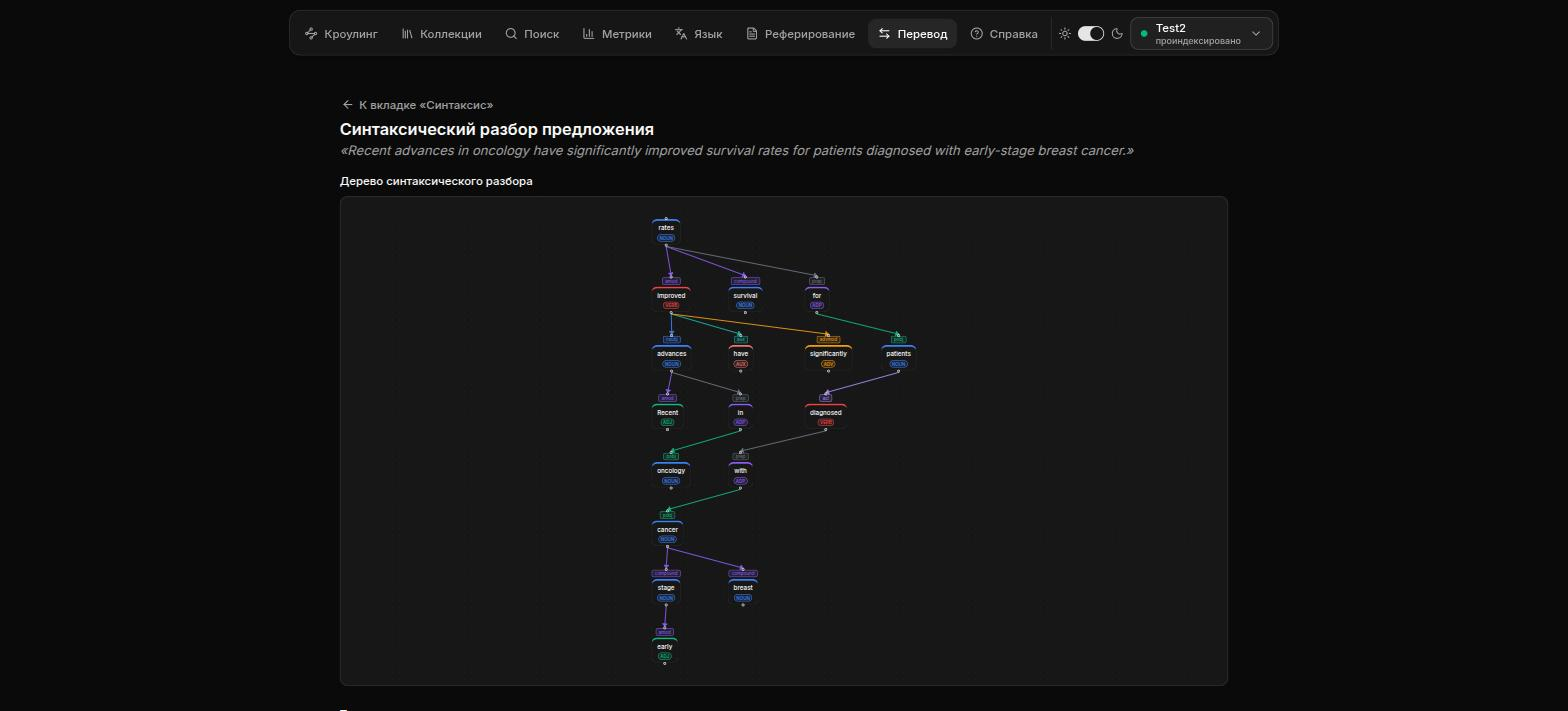
\includegraphics[width=0.75\textwidth]{lab/pictures/syntax_tree.png}
  \caption{Вкладка «Синтаксис»: дерево синтаксического разбора выбранного предложения}
  \label{fig:syntax-tree}
\end{figure}

\begin{figure}[H]
  \centering
  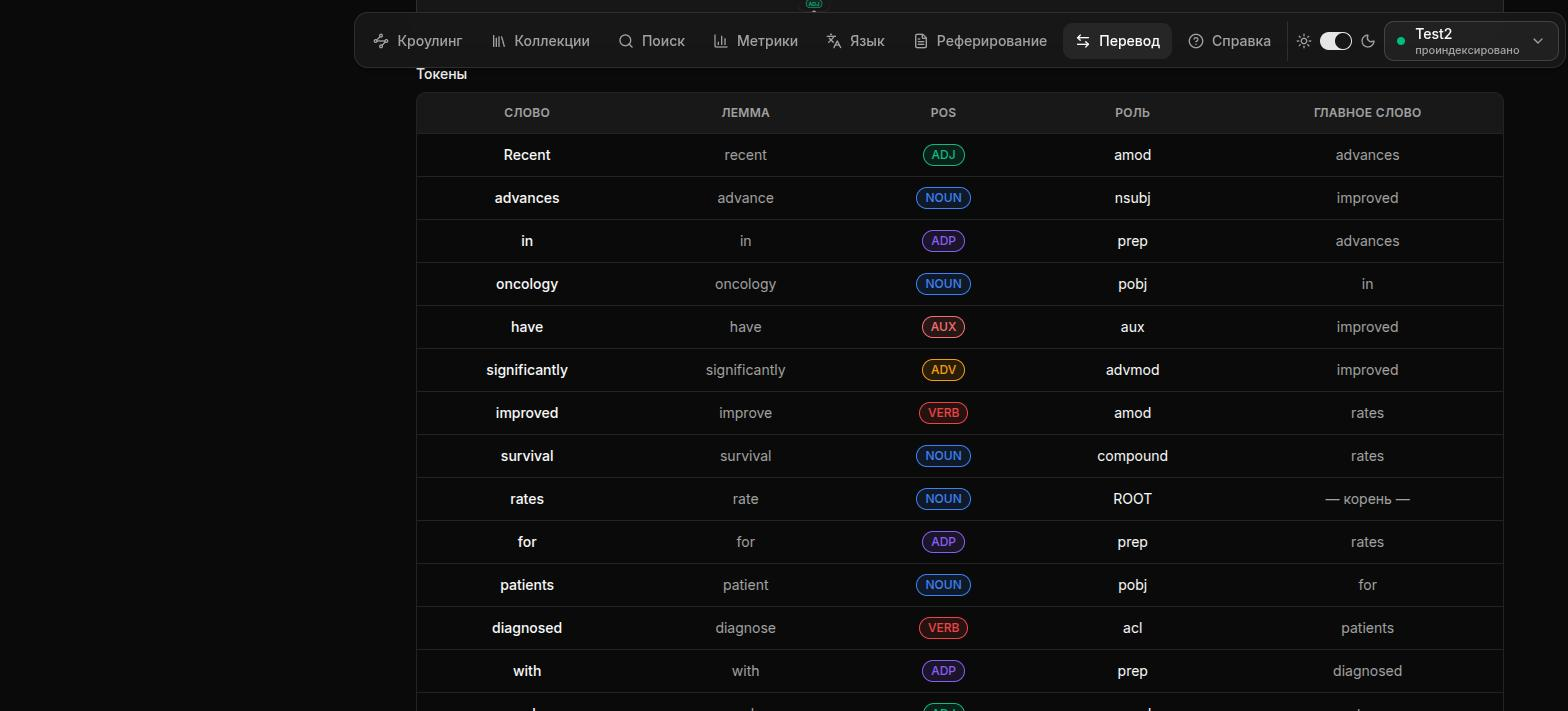
\includegraphics[width=\textwidth]{lab/pictures/syntax_tokens.png}
  \caption{Таблица токенов под деревом разбора: слово, лемма, POS, синтаксическая роль, главное слово}
  \label{fig:syntax-tokens}
\end{figure}

\textbf{Частотный список слов (вкладка 1).} Функциональность ЛР1
весеннего семестра (частотный список слов) переиспользована
буквально -- та же функция токенизации с исключением стоп-слов, что и
для индексации документов, только результат группируется по (лемма,
POS) и сортируется по убыванию частоты, а не используется для
TF-IDF. Каждое слово в списке сопровождается переводом, найденным тем
же словарём и по тому же правилу отката, что и в основном переводе
(рисунок~\ref{fig:word-list}).

\begin{figure}[H]
  \centering
  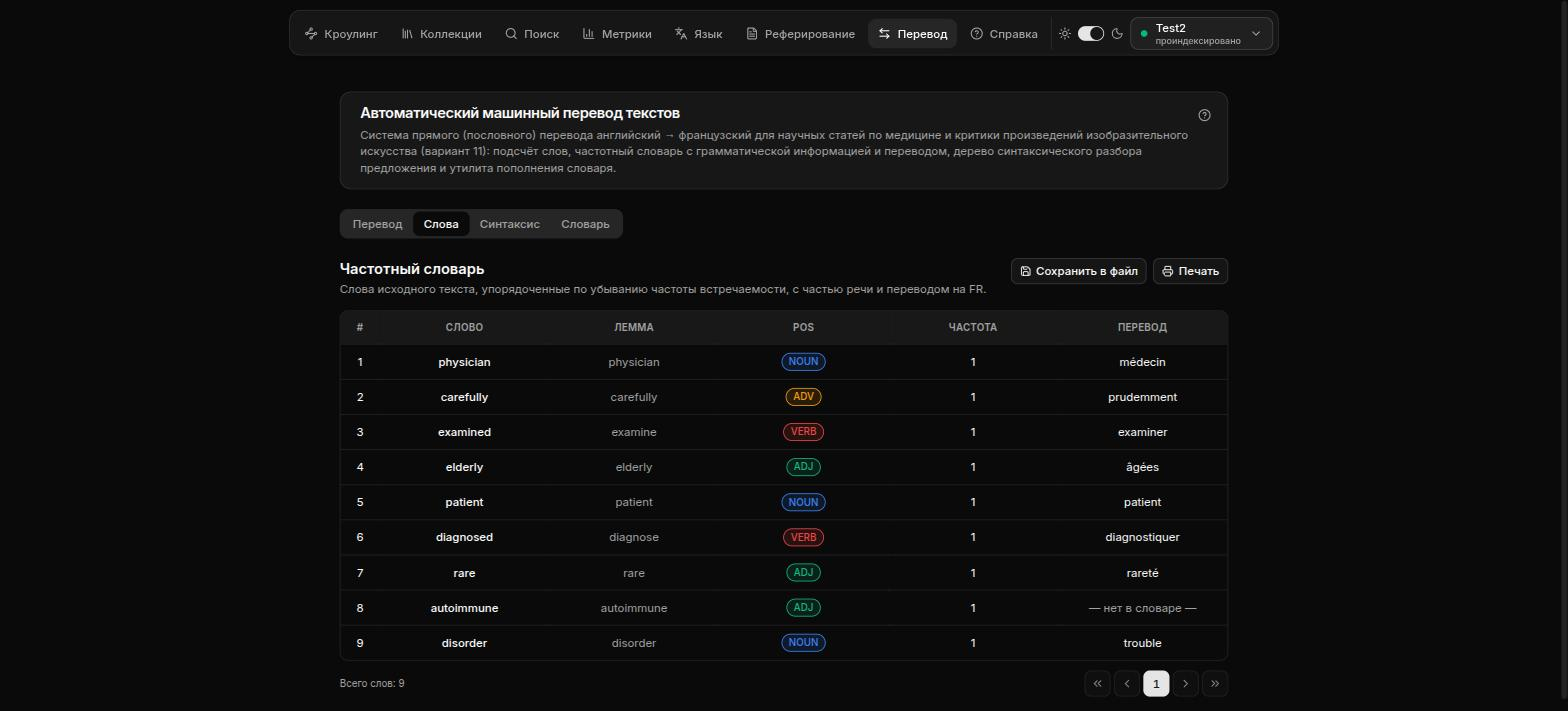
\includegraphics[width=\textwidth]{lab/pictures/word_list_tab.png}
  \caption{Вкладка 1: частотный список слов с частью речи и переводом; слово \emph{autoimmune} отсутствует в словаре и явно помечено}
  \label{fig:word-list}
\end{figure}

\textbf{Сохранение и восстановление регистра, пунктуации и пробелов.}
Токенизация spaCy используется не только для лемматизации, но и для
точной реконструкции текста: у каждого токена берётся
\texttt{whitespace\_} (пробел/перевод строки после токена, как он был
в исходном тексте), поэтому пунктуация и форматирование переведённого
текста совпадают с исходным без дополнительной постобработки; регистр
первой буквы и полностью заглавные слова переводного эквивалента
подстраиваются под регистр исходного слова.

\begin{figure}[H]
  \centering
  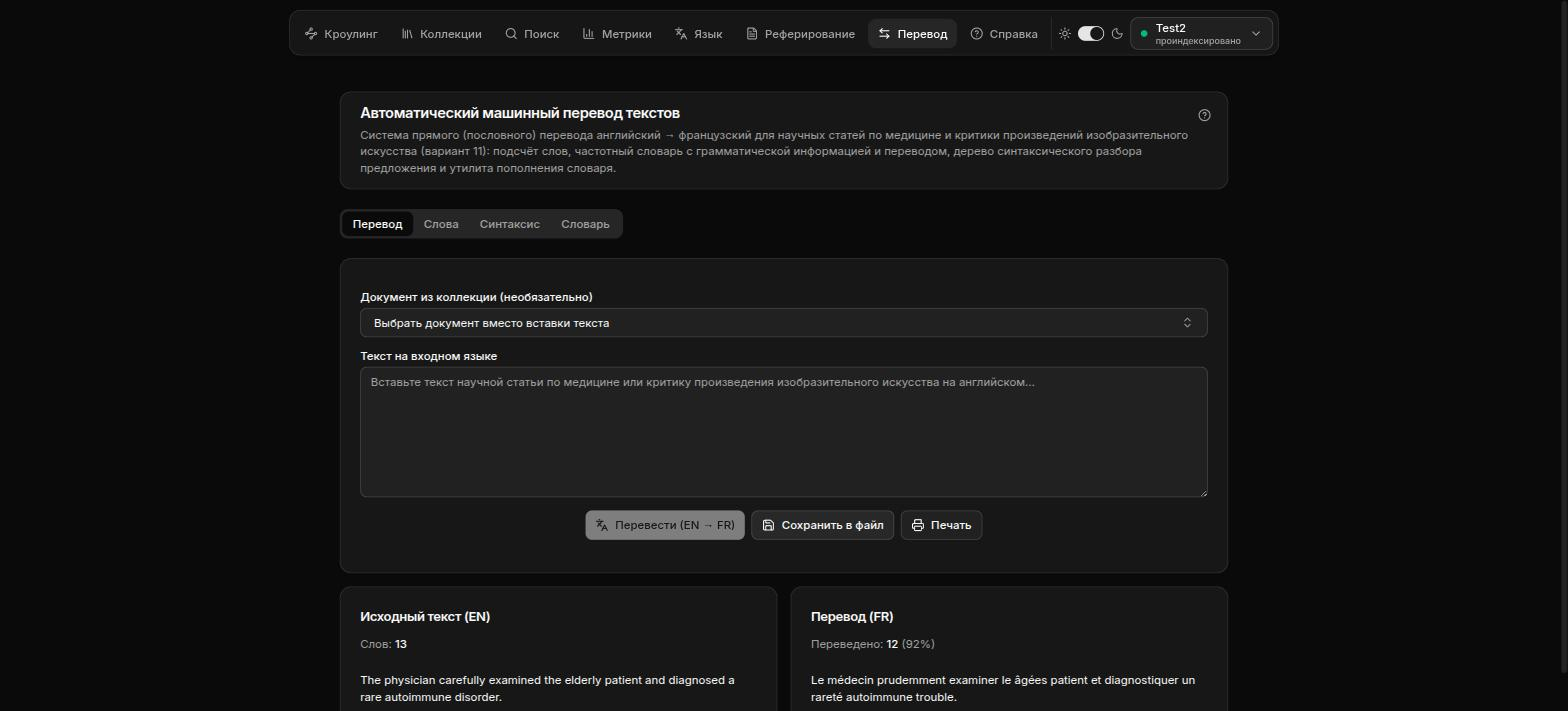
\includegraphics[width=\textwidth]{lab/pictures/translation_tab.png}
  \caption{Вкладка «Перевод»: количество слов и процент переведённых слов вынесены в заголовки карточек исходного текста и перевода}
  \label{fig:translation-tab}
\end{figure}

\labpartbreak{Утилита пополнения и корректировки словаря}

Отдельная вкладка «Словарь» -- утилита, явно требуемая методичкой
(«обеспечить наличие утилиты автоматического пополнения/корректировки
полученного словаря (таблицы БД)»): постраничная таблица всех статей
словаря с поиском по слову или переводу, добавлением новой статьи
(лемма, часть речи -- выбор из списка тегов spaCy или «любая», перевод,
примечание) и редактированием/удалением существующей
(рисунок~\ref{fig:dictionary-tab}). Добавление заведомого дубликата
(та же лемма, тот же язык и та же часть речи) отклоняется с кодом 409
-- отдельно проверено, что это работает и для часового-значения
\texttt{"*"} (см. предыдущий раздел про \texttt{NULL}).

\begin{figure}[H]
  \centering
  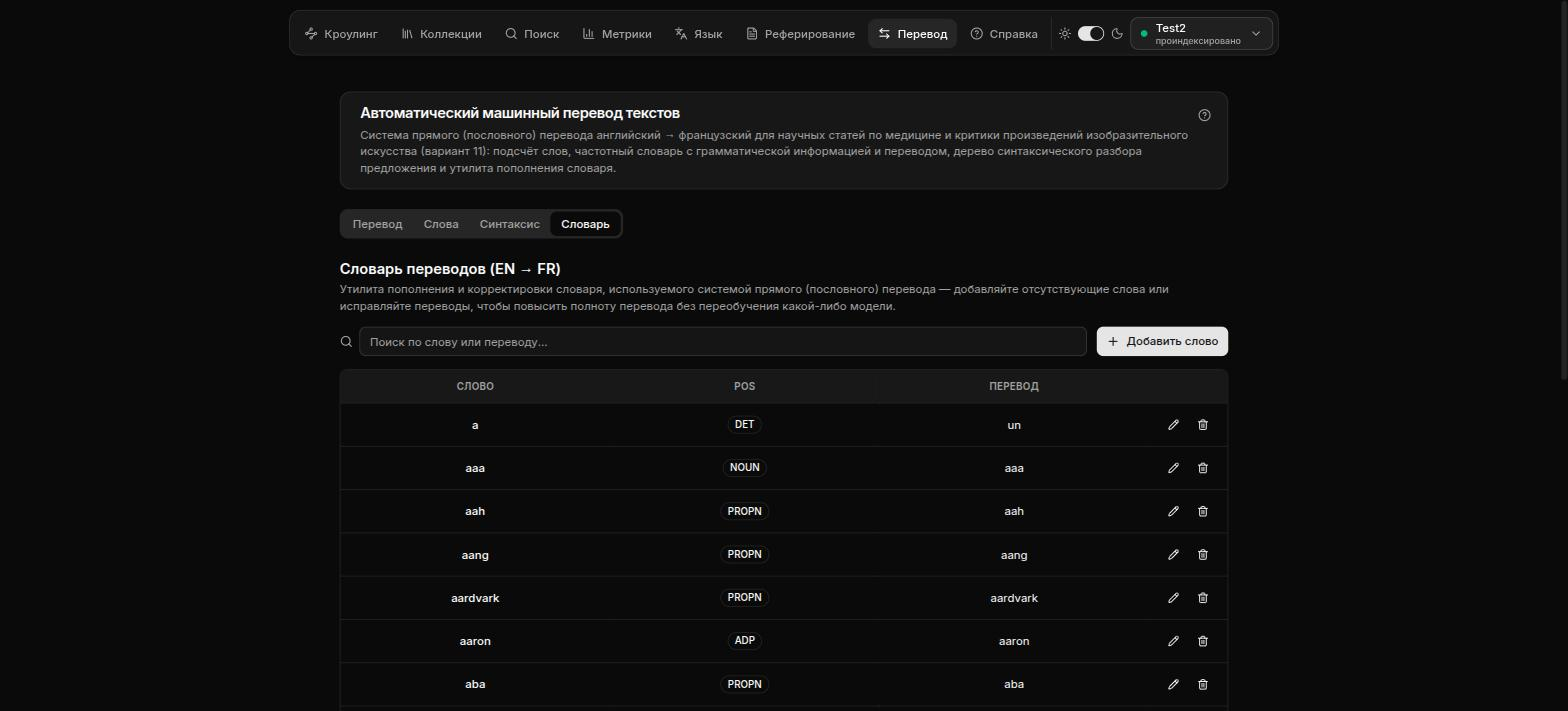
\includegraphics[width=\textwidth]{lab/pictures/dictionary_tab.png}
  \caption{Вкладка «Словарь»: постраничная таблица статей словаря переводов с POS-тегами}
  \label{fig:dictionary-tab}
\end{figure}

\labpartbreak{Тестовые тексты предметной области}

Вариант 11 задаёт направление перевода англо-французское и предметную
область -- научные статьи по медицине и критика предметов
изобразительного искусства. Для тестирования подготовлено по одному
характерному тексту каждой области (наукообразный абзац о клиническом
исследовании в онкологии -- 98 слов; искусствоведческий абзац о
выставке современной живописи -- 107 слов), не входящих в исходные
данные, на которых строился словарь (см. далее) -- это тексты именно
той тематики, для которой методичка требует оценить полноту перевода.

\labpart{Результаты тестирования и оценка качества}

\textbf{Пополнение словаря реальными данными.} Стартовый вручную
курируемый словарь (служебные слова английского языка, общая научная
лексика и порядка 100 терминов медицины/искусствоведения) содержал
всего 311 статей и переводил лишь около половины слов реального
текста предметной области (таблица~\ref{tab:dictionary-coverage}).
Он был расширен реальным двуязычным словарём MUSE (Facebook Research,
113~286 пар слов), отфильтрованным до топ-50~000 самых частотных слов
английского языка (по корпусу субтитров hermitdave/FrequencyWords) --
это отсекло длинный хвост из имён собственных, топонимов и
аббревиатур, случайно попавших в MUSE вместе с полезной лексикой.
Каждое из оставшихся 33~960 слов размечено частью речи \emph{вне
контекста предложения} через тот же конвейер spaCy (пакетно, единым
проходом \texttt{nlp.pipe}); итоговый словарь -- 34~050 статей.

\begin{table}[H]
  \centering
  \caption{Полнота перевода тестовых текстов предметной области до и после пополнения словаря}
  \label{tab:dictionary-coverage}
  \begin{tabularx}{\textwidth}{|X|r|r|r|}
    \hline
    Словарь & Статей & Медицинский текст & Искусствоведческий текст \\
    \hline
    Только курируемый (стартовый) & 311 & 54/98 слов (55{,}1\,\%) & 78/107 слов (72{,}9\,\%) \\
    \hline
    Курируемый + MUSE (топ-50к слов) & 34~050 & 93/98 слов (94{,}9\,\%) & 106/107 слов (99{,}1\,\%) \\
    \hline
  \end{tabularx}
\end{table}

Оставшиеся непереведёнными слова в обоих текстах -- узкоспециализированные
термины вне топ-50~000 частотных слов языка (например,
\emph{autoimmune} в медицинском тексте, рисунок~\ref{fig:word-list}) --
ожидаемый результат для системы прямого перевода: её словарь конечен
по построению, и утилита пополнения словаря (см. выше) -- предусмотренный
методичкой способ закрыть именно такие случаи вручную, не переобучая
никакую модель.

\textbf{Время выполнения.} Перевод обоих тестовых текстов (98 и 107
слов) занял 78{,}6~мс и 75{,}6~мс соответственно, включая обращение к
\texttt{nlp-service} по HTTP; построение словаря lookup из 34~050
записей БД при каждом переводе не кешируется и укладывается в то же
время -- отдельного узкого места по производительности на текстах
такого объёма не выявлено.

\labpart{Анализ результатов и предложения по улучшению}

\begin{enumerate}
  \item \textbf{Размер словаря -- определяющий фактор качества системы
  прямого перевода.} Рост словаря в 109 раз (с 311 до 34~050 статей)
  поднял полноту перевода тестовых текстов с 55--73\,\% до 95--99\,\%
  (таблица~\ref{tab:dictionary-coverage}) при том, что сам алгоритм
  перевода не менялся -- для систем этого класса словарь, а не
  правило подстановки, является узким местом качества, что прямо
  следует из определения пословного перевода в методичке.
  \item \textbf{POS-тегирование словаря вне контекста предложения --
  компромисс, а не идеальное решение.} Присвоение одной части речи
  каждому слову словаря (без учёта контекста, в котором оно встретится
  в переводимом тексте) неизбежно даёт часть словаря с «неверной» на
  первый взгляд частью речи для конкретного предложения; это компенсируется
  откатом по маске \texttt{"*"} (см. выше), ценой которого является то,
  что для омонимов с разным переводом в разных частях речи (например,
  существительное и глагол с общим написанием) может быть выбран
  перевод не той формы. Хранение нескольких переводов на лемму
  (а не одного, выбираемого правилом отката) устранило бы эту
  проблему ценой усложнения структуры словаря и интерфейса его
  редактирования.
  \item \textbf{Что можно добавить в систему для её улучшения.}
  \begin{itemize}
    \item согласование словоформы перевода с исходным словом (число,
    время, падеж) -- сейчас переводной эквивалент подставляется в
    начальной форме, взятой из словаря, без склонения/спряжения под
    грамматическую форму исходного слова;
    \item кеширование lookup-словаря между запросами перевода (сейчас
    все 34~050 записей перечитываются из БД при каждом переводе) --
    ускорило бы обработку текстов на коллекциях с частыми повторными
    переводами;
    \item статистика по словарю (доля непереведённых слов по
    последним $N$ переводам) прямо на вкладке «Словарь» -- подсказывала
    бы, какие слова стоит добавить в первую очередь, вместо ручного
    просмотра частотного списка после каждого перевода;
    \item предметно-ориентированные дополнения словаря (аннотированные
    списки терминов конкретно по онкологии, кардиологии, критике
    живописи и т.\,д.) вместо общего словаря топ-50~000 слов --
    подняли бы полноту перевода специализированной лексики предметной
    области варианта без раздувания словаря общеупотребительными
    словами, которых там уже достаточно.
  \end{itemize}
  \item \textbf{Где систему можно применить.}
  \begin{itemize}
    \item черновой перевод документов информационно-поисковой системы
    ЛР1 для быстрого ознакомления с содержанием перед выбором, читать
    ли документ полностью на исходном языке;
    \item учебный полигон для сравнения с более сложными архитектурами
    машинного перевода (системы с трансфером, нейросетевые модели) --
    прямой перевод даёт понятную базовую линию качества и явно
    показывает, какие именно случаи (согласование форм, многозначные
    слова, отсутствующая лексика) требуют более сложной модели;
    \item источник частотного словаря предметной области (вкладка~1)
    как самостоятельный инструмент -- например, для быстрой оценки
    того, насколько текст на входном языке относится к уже освоенной
    словарём терминологии.
  \end{itemize}
\end{enumerate}

\labpartbreak{Использованные готовые компоненты}

\begin{table}[H]
  \centering
  \caption{Библиотеки, готовые данные и программные средства, использованные при реализации ЛР4 (дополнительно к перечисленным в отчётах по ЛР1--ЛР3)}
  \label{tab:stack-translation}
  \small
  \begin{tabularx}{\textwidth}{|l|X|}
    \hline
    Компонент & Назначение \\
    \hline
    spaCy (теггер и парсер) & POS-теги для частотного словаря и
      перевода (теггер \texttt{en\_core\_web\_sm}, без изменений
      переиспользован из ЛР3) и дерево зависимостей для вкладки~2
      (парсер, для основного конвейера индексации отключаемый ради
      скорости, здесь включается отдельно). \\
    \hline
    MUSE (Facebook Research) & Источник реального двуязычного словаря
      en--fr (113~286 пар слов, \texttt{github.com/facebookresearch/}
      \texttt{MUSE}) для пополнения стартового курируемого словаря. \\
    \hline
    FrequencyWords (hermitdave) & Список топ-50~000 слов английского
      языка по частоте в корпусе субтитров
      (\texttt{github.com/hermitdave/FrequencyWords}) -- фильтр для
      отсечения имён собственных/топонимов/аббревиатур из MUSE. \\
    \hline
    reactflow & Визуализация дерева синтаксического разбора (вкладка~2)
      -- перенос идеи компонента \texttt{DependencyGraph} из
      \texttt{corpus-manager}, переписанного под текущий UI-кит проекта. \\
    \hline
  \end{tabularx}
\end{table}
